\chapter{機械}
NHKロボコンにおいて機械の出来はそのチームの成績を大きく左右します. そのため, いかに性能を発揮できる機械を作れるかが鍵となります. 
\section{全体構成}\label{mecha:base}
NHKロボコンのロボットは大きく以下の3つの部位に分類できます.
\begin{itemize}
    \item 足回り
    \item 把持機構
    \item 投擲機構
\end{itemize}
このうち足回りはほとんどすべての競技に用いられる最も基本的な構造単位です. 把持機構や投擲機構は, 競技によっては直接用いることがない場合もありますが, どちらかの機構は必要になるでしょう. いずれにせよ, この3つの機構がロボットを設計する上で基礎的な事項となるので, しっかりとおさえておきましょう. 
\subsection{足回り}
ロボコンに用いられる足回りはいくつかの種類に分類できます. ここでは, それぞれの足回りについて特徴を紹介していきます.

\subsubsection{オムニホイール}
オムニホイールは, 図\ref{fig:omuni_round}に示すような主軸を中心とする回転部品の外周上に, 主軸方向に回転する複数の受動車輪がついた構造となっています. そのため, 主軸の回転方向には力を伝え, その主軸方向には力を逃がすようになります. この車輪を複数使用することで, 全方向に移動出来るロボットを作る事ができます. 一般に2次元平面上を動かす場合であれば, 2方向の向きと回転を制御できれば良いので, 3つ以上のオムニホイールを適切に配置すれば全方向に移動できるロボットを制作できます. 比較的簡単に全移動方向を実現でき制御難度も低いので, ロボコンにおいては多く用いられます. 

\begin{figure}[h]
  \centering
  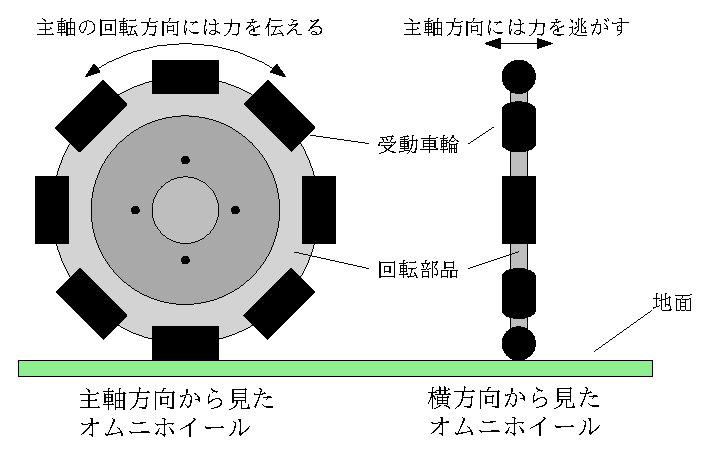
\includegraphics[width=10cm]{mecha/fig/omuni.eps}
  \caption{オムニホイールの構造}
  \label{fig:omuni_round}
\end{figure}

よく用いられる構成として, 図\ref{fig:3-omuni}のように3つのオムニホイールを正三角形の頂点に配置するものや, 図\ref{fig:4-omuni}4つのオムニホイールを正方形の頂点に配置するものがありますが, これ以外の構成でも3自由度が確保できるような構成であれば全方向移動するロボットを制作することができます. 
例えば図\ref{fig:4-omuni-po}のようにひし形の構成も可能です. しかし, 図\ref{fig:fiji}のように4つのオムニホイールを平行に並べてたような構成は1方向の移動と回転しか行えないため, 全方向移動は不可能です. このような場合は, 図\ref{fig:fiji_imp}のようにもう一方向に移動できる車輪を付け加えることで全方向移動が可能となります.

\begin{figure}[h]
 \begin{minipage}{0.5\hsize}
  \begin{center}
   \includegraphics[width=50mm]{mecha/fig/3-omuni.eps}
  \end{center}
  \caption{代表的な3輪オムニ配置}
  \label{fig:3-omuni}
 \end{minipage}
 \begin{minipage}{0.5\hsize}
  \begin{center}
   \includegraphics[width=50mm]{mecha/fig/4-omuni.eps}
  \end{center}
  \caption{代表的な4輪オムニ配置}
  \label{fig:4-omuni}
 \end{minipage}
\end{figure}

\begin{figure}[h]
  \centering
  \includegraphics[width=7cm]{mecha/fig/4-omuni-po.eps}
  \caption{変則的なオムニホイールの配置}
  \label{fig:4-omuni-po}
\end{figure}

\begin{figure}[h]
 \begin{minipage}{0.5\hsize}
  \begin{center}
   \includegraphics[width=50mm]{mecha/fig/fiji.eps}
  \end{center}
  \caption{オムニホイールが平行に4つ並んでいる機体}
  \label{fig:fiji}
 \end{minipage}
 \begin{minipage}{0.5\hsize}
  \begin{center}
   \includegraphics[width=50mm]{mecha/fig/fiji_imp.eps}
  \end{center}
  \caption{オムニホイールを付け足した例}
  \label{fig:fiji_imp}
 \end{minipage}
\end{figure}

注意点として, 全方向移動が出来るといっても, 形状によって方向によって速度の出しやすさ, トルクの出しやすさが異なります. ちなみに図\ref{fig:3-omuni},\ref{fig:4-omuni}のようなロボットの場合は最も速度及びトルクが出しやすいのは回転方向です. また, 接地点に関しても注意が必要です. 平面は3点で定まるので, 接地点が3つの場合は必ずすべての車輪が接地するため問題がないですが, 接地点が4つ以上ある場合, 地面の状況によってはすべての車輪が接地しない可能性があります. 接地しない車輪があると, その車輪は空回りをしてしまい, うまくロボットを制御出来なくなってしまうので, 必ずすべての車輪が接地するようにしなくてはいけません. ロボコンのフィールドは平坦であるので, 多くの場合は問題になりませんが, 足回りのフレームが過剰に硬いとうまく接地しないこともあります. 足回りのフレームはある程度柔らかいほうがこれらのトラブルを避けやすい
です. 
バネなどを用いて車輪を地面に押し付けてすべての車輪を接地させる方法もありますが, 機構が複雑になるほか, ばね定数等を適切に設定しないと振動の原因となってしまうのであまり推奨できません. 

\subsubsection{メカナムホイール}
メカナムホイールはオムニホイールと似ていますが, 図\ref{fig:mechanum_round}のように本体外周上についているローラーが, 本体に対して45$^{\circ}$傾いています. このホイールを図\ref{fig:mechanum}のように4つ配置することで, 全方向移動するロボットを制作できます. 

\begin{figure}[h]
  \centering
  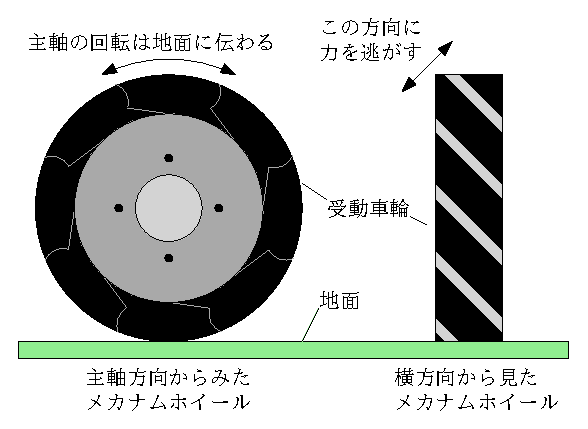
\includegraphics[width=10cm]{mecha/fig/mecanum.eps}
  \caption{メカナムホイールの構造}
  \label{fig:mechanum_round}
\end{figure}

\begin{figure}[h]
  \centering
  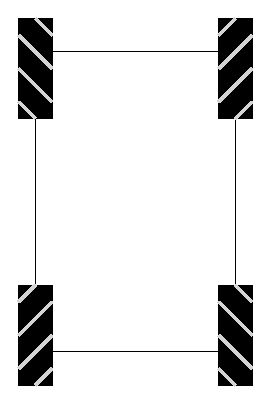
\includegraphics[width=5cm]{mecha/fig/fiji_mechanam.eps}
  \caption{メカナムホイールの配置}
  \label{fig:mechanum}
\end{figure}
基本的な事項はオムニホイールと同じですが, メカナムホイールは直進方向への運動性能が高いことが特徴です. その他, オムニホイールを用いるより足回りのフレームを組みやすいというメリットもあります. 

\subsubsection{独立二輪}
この足回りは, 通常の車輪を駆動輪として用います. 
図\ref{fig:sadou2}のように2つの駆動輪から成りますが, それだけでは機体を支えることができないのでキャスタなどを用います. この機体の特徴として, オムニホイールやメカナムホイールを用いたロボットと異なり, 全方向移動が出来ないことが挙げられます. 行きたい方向に行くには, その方向に機体の向きを変えてから移動する必要があります. このような機体は全方向移動出来る機体に比べて制御が難しくなります. 

\begin{figure}[h]
  \centering
  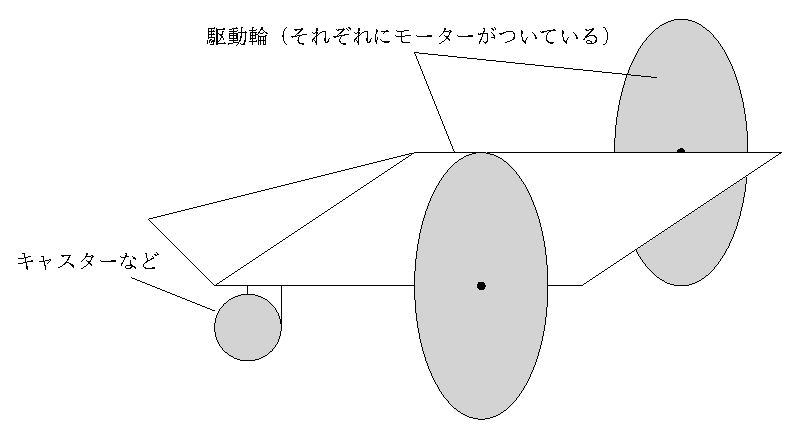
\includegraphics[width=10cm]{mecha/fig/sadou2.eps}
  \caption{代表的な独立二輪の配置}
  \label{fig:sadou2}
\end{figure}

オムニホイールやメカナムホイールと比べて車輪の制作や改良がしやすいため, より運動性能の高い機体を作りやすいというメリットがあります. また, 必要となるモーターが2つで済むため, 機体重量を軽量化できるという点もメリットです. 一方で機体の設計が難しいという問題があります. 独立二輪の機体で性能を発揮するためには駆動輪を必ず接地させる必要があります. 可能であればキャスターを1つにすれば接地の観点では最も良いですが, 安定性に劣ります. 一方でキャスターを2つ以上つけると安定性の観点では優れますが, うまく駆動輪が接地しない場合もあります. 
また, 急加速をした際にも機体が安定しているためには, 駆動輪が進行方向に対して中央にあるのが望ましいですが, その場合はキャスターを4つつけることとなります. この場合, より駆動輪の接地が難しくなるため, 設計段階からより注意が必要です. 

\subsubsection{独立四輪}
この足回りは長方形状の機体の各頂点に進行方向に並べられた4つの駆動輪から成ります. 
独立二輪と同じく, 車輪の制作や改良がしやすいというメリットがあるが, 旋回性能では大きく劣ります. 左右の車輪の回転速度の制御により, 若干の方向転換は可能でありますが, 基本的には直進性能を突き詰めたような足回りです. 一般的な競技には用いられないですが, 稀に存在するほとんど直進しか必要のない競技において用いられる場合があります. 

\subsubsection{独立ステアリング(swerve drive)}
通常のタイヤがそれぞれ方向転換出来るようになっていて, 進行方向に向けてタイヤの向きを変えることにより, 全方向への移動を実現します. こちらも通常のタイヤを用いるため, 車輪の制作や改良がしやすく, 独立二輪と同様運動性能の高い機体を作りやすいというメリットがあります. 

一方で, 車輪を二つの軸で回転させる必要があるため, 機構が複雑になり, 設計やメンテナンスが困難となるというデメリットがあります. 制御の難易度は機体の構成によって変わるので一概には言えないですが, ロボコンで多く用いられる車軸と旋回軸が同一平面上にあるタイプの機体は独立二輪と同程度の難易度です. 
ただし, これはすべての足回りにおいて言えることですが, より高い速度や加速度を出そうとするとより制御は難しくなります. 

\subsection{把持機構}
NHKロボコンにおいてフィールド上にあるオブジェクトを回収したり, オブジェクトを指定の位置に運搬するというのは非常に多く見られる課題です. 
そのため, オブジェクトの把持はロボコンにおいて非常に重要となります. 実際にオブジェクトを掴んで運搬するようなタスクがない競技であっても, オブジェクトを全く扱わない競技は稀であるため, 把持機構の考え方などは役に立つことがあります. 

尚, オブジェクトを運搬するだけならば引きずって運搬するという手段もあるという点は頭に入れておきましょう. ただしルールなどで禁止されている場合も多いですのでルールはよく確認しましょう. 

さて, ここではロボコンでオブジェクトの把持に用いられる機構を3つに分けて紹介します. 

\subsubsection{ハンドによる把持}
この手法は図\ref{fig:hand}に示すように2つもしくはそれ以上の方向からオブジェクトを挟むことで把持します. 
アクチュエータとしてはサーボモーターやエアシリンダなどを用いたものがロボコンでは多く見られます. 
把持する物体が同じであっても様々な種類や構造が考えられるため, ここでは個々のハンドを取り上げて解説はしません. 
インターネット等で調べれば様々なハンドを見つけることが出来るので, 各自調べて参考にしてください. 

\begin{figure}[h]
  \centering
  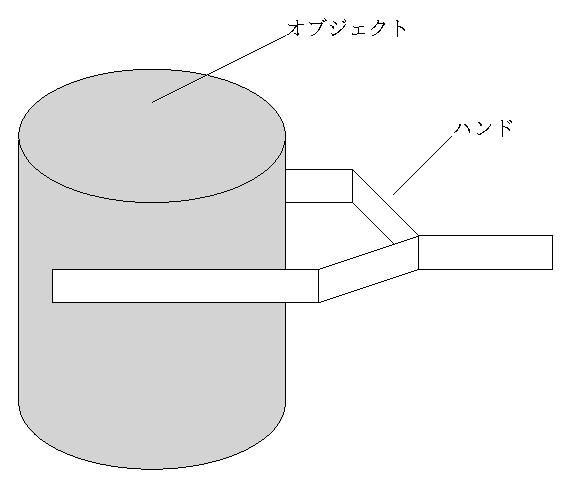
\includegraphics[width=7.5cm]{mecha/fig/hand.eps}
  \caption{ハンドによる把持の例}
  \label{fig:hand}
\end{figure}

ここで, ロボコンにおいて重要となるのはオブジェクトに対して最適化することです. 一般的に用いられるハンドはできるだけ多くの種類の物体を把持できるよう設計されていますが, ロボコンでは一つの種類のオブジェクトをつかめれば十分である場合が多いので, 目的のオブジェクトに特化したハンドを制作したほうが有利です. 
オブジェクトにふれる部分の形状や素材をオブジェクトに合うように設計, 改良して素早く, 正確にオブジェクトを把持できるようにすると, 競技を有利に進められる場合が多いです. 

メリットとしては確実にオブジェクトをつかめて信頼性が高いこと, 改良が施しやすいことなどが挙げられるが, オブジェクトが大きくなるとハンドも大きく, 重くなりやすいというデメリットもあります. 
\subsubsection{吸引パッドによる把持}
この手法は対象のオブジェクトを図\ref{fig:vacuum}のように吸引パッドなどを用いて吸着することで把持します. 
一般的には吸引パッドからポンプにつながっており, ポンプでオブジェクトと吸引パッドの間の空気を抜くことでオブジェクトを把持します. 
ロボコンではポンプではなくダクテッドファンを用いてこの吸引を行う場合もあります. 

\begin{figure}[h]
  \centering
  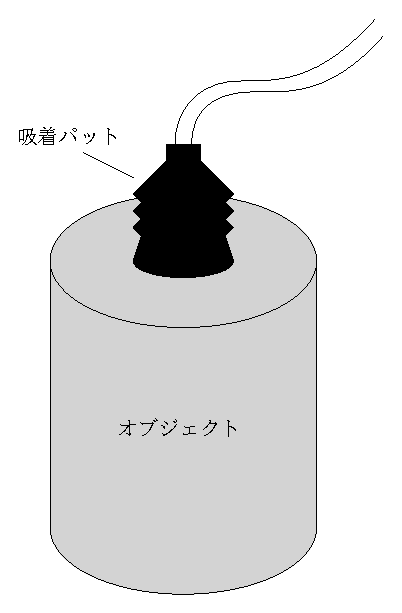
\includegraphics[width=5cm]{mecha/fig/vacuum.eps}
  \caption{吸引パッドによる把持の例}
  \label{fig:vacuum}
\end{figure}

吸引パッドを用いた把持方法は産業界でも多く用いられており, 様々な種類の吸着パッドが各メーカーから販売されています. オブジェクトによって適した吸着パッドは異なるのでメーカーの説明などを参考に適した吸着パッドを選ぶことが重要となります. 

メリットとしてはオブジェクトに吸引パッドがふれるだけで把持が行えるため機構が簡単になり, 様々なオブジェクトに対応できるという点があります. 
一方デメリットとして重いオブジェクトを把持することに適していないことや, オブジェクトの表面性状によっては使用できないこともある点です. 特にオブジェクトの表面性状に関しては注意が必要で, 練習用のオブジェクトでは把持できたが本番のオブジェクトでは把持できなかったという事象も起こりやすいので, 採用の際には十分な調査, 検証をおすすめします. 
\subsubsection{オブジェクトの形状に合わせた把持}
この手法は使用できるとは限りませんが, 使用できれば大きなメリットとなる可能性のある方法です. 
例えば図\ref{fig:advance}のように穴の空いているオブジェクトであれば棒状をアームを差し込んで引っ掛けて把持したり, 引っかかりうる部位のあるオブジェクトであれば鉤爪状のものを引っ掛けて把持したりすることが出来ます. 

\begin{figure}[h]
 \begin{minipage}{0.5\hsize}
  \begin{center}
   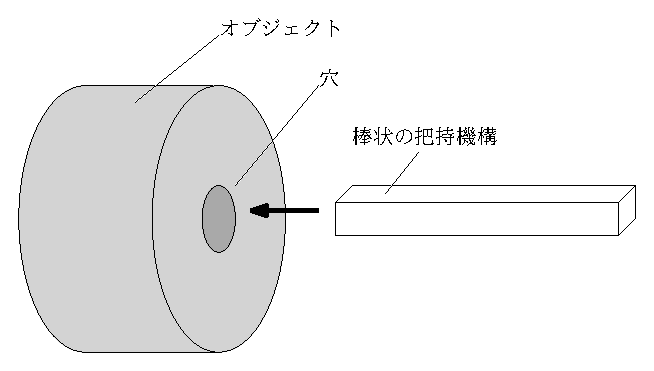
\includegraphics[width=75mm]{mecha/fig/hole.eps}
  \end{center}
 \end{minipage}
 \begin{minipage}{0.5\hsize}
  \begin{center}
   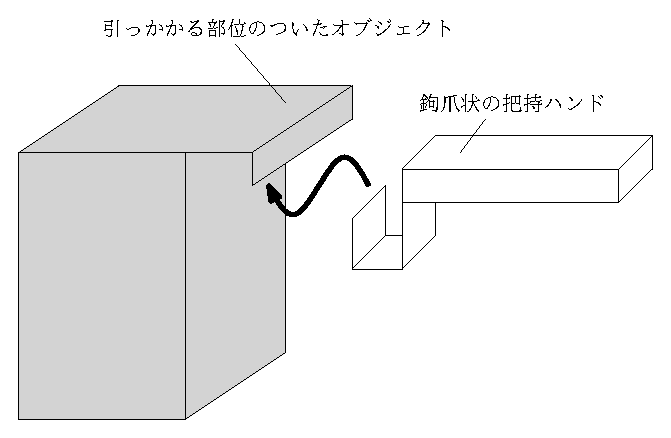
\includegraphics[width=75mm]{mecha/fig/kagi.eps}
  \end{center}
 \end{minipage}
 \caption{オブジェクトの形状を利用した把持の例}
 \label{fig:advance}
\end{figure}

これらの方法は使用するオブジェクトの形状や特性に大きく依存しており, このような形状であれば使用できる, 使用したほうが有利となる, という明確な答えはありません. 
しかしながら上記のハンドや吸着パッドを用いる方法よりも簡単に把持できたり素早く把持出来たりする場合は上記2つの手法に対して大きなアドバンテージとなります. ロボコンの「アイディアで魅せられる」部分でもあるので, 使用するオブジェクトをよく分析して上記2つの方法でない何か良い把持方法がないか考えることもアイディア会議の段階では大切にしましょう.
\subsection{投擲機構}
投擲は競技によっては全く必要のない場合もある一方で, 近年のNHKロボコンでは投擲が必要なルールが増えてきています. 投擲は難しい部分でもあり, 差が出やすい部分でもあるので設計段階から重要となる部分です. 

投擲の際に詰まるポイントとしてよくあるのは, 飛距離が出ないことと正確性が確保出来ないことです. 競技によっては正確性が問題とならない場合もあるものの, 多くの場合は目標の位置を通過もしくは着地するようにオブジェクトを投擲する必要があり, 毎回正確に目標位置に投擲ができなくてはいけません. 
飛距離に関してはオブジェクトに対して適切なエネルギーを与える必要がありますが, 機械の強度が不足していたりアクチュエーターの選定が不十分であると必要なエネルギーをオブジェクトに与えることが出来ません. 正確性に関しては投擲機構自体に正確性が低い場合もありますが, それ以外の要素も加わってくるので注意が必要となります. 代表的なものが足回りで, 毎回同じ位置に停止できるか, 角度にずれはないかなどが投擲の結果を左右します. この問題には足回りをどの程度ずれているかを正確に計測して目標の位置に正確に制御する技術等で対処することが多いですが, 壁などを利用してロボットを押し当てて位置や向きを修正するという方法もあります. 
他にも, オブジェクトと投擲機構によってはそれらの性質などが投擲結果の正確性に関わってくることもあります. このあたりはオブジェクトの形状や特性によっても変わってくるので実験を繰り返してデーターを集め, 原因を突き止めて修正していくことが重要となります. 

さて, 投擲に関してはオブジェクトの形状や重量などによって多数の方法が考えられますが, 今回は比較的多くのオブジェクトに適応できる例に絞って紹介します. 
\subsubsection{ベルト・ローラー型}
図\ref{fig:roller}に示すようにオブジェクトに2方向もしくはそれ以上の方向から回転するベルトもしくはローラーを押し当ててオブジェクトを加速, 射出します. 野球などのピッチングマシーンでも同様の仕組みが用いられています. ローラーやベルトによって与えるエネルギーによってオブジェクトを投擲するため, ローラーやベルトからスムーズにエネルギーを伝えられるかが鍵となります. 
ローラーやベルトがオブジェクトに対して滑ってしまうとエネルギーの伝達がスムーズに行かないので, ローラーやベルトの性能が重要となってきます. 

\begin{figure}[h]
  \centering
  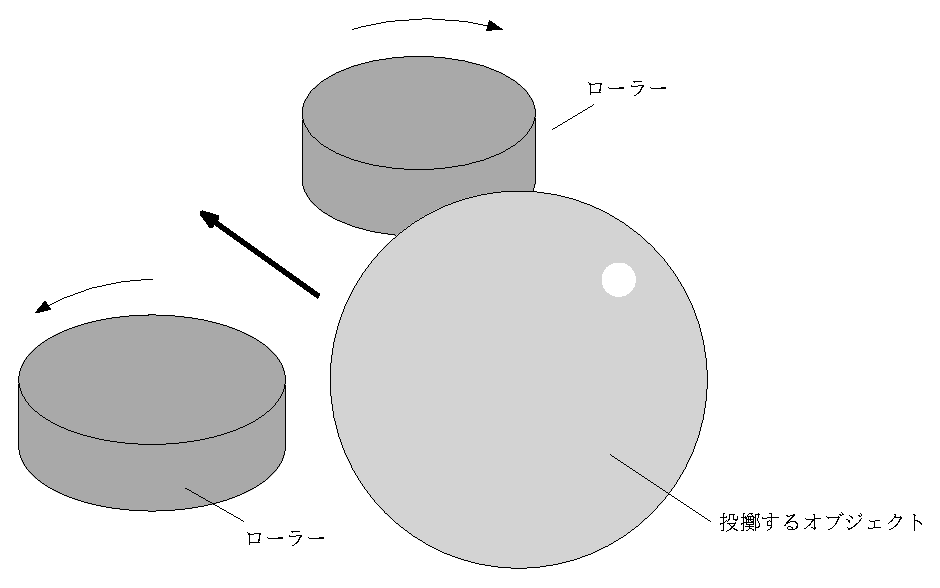
\includegraphics[width=10cm]{mecha/fig/roller.eps}
  \caption{ベルト・ローラー型の投擲機構}
  \label{fig:roller}
\end{figure}

比較的簡単に制作でき, オブジェクトの装填から射出までがスムーズであるというメリットがありますが, 柔らかいオブジェクトの投擲には向いていません. 
\subsubsection{直動カタパルト型}
図\ref{fig:cataput}のように直線上に高速に動く台などの上に投擲したいオブジェクトをセットし, 台とオブジェクトを加速した後, オブジェクトを台から分離することで投擲を行います. 
直動機構の性質上, 加速距離が限られるため, 非常に素早く加減速を行う必要があります. 
そのため機械的な負荷が大きく, アクチュエーターの選定や機構の設計などには注意が必要です. 

\begin{figure}[h]
  \centering
  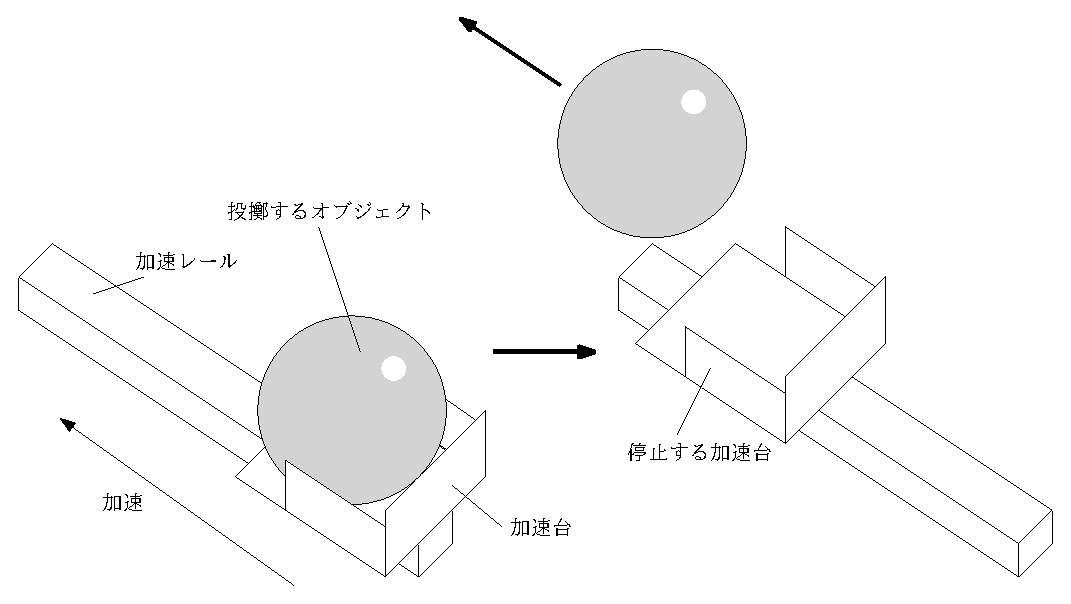
\includegraphics[width=15cm]{mecha/fig/catapult.eps}
  \caption{直動カタパルト型の投擲機構}
  \label{fig:cataput}
\end{figure}

機構自体の仕組みは単純であるものの, 競技によってはオブジェクトを装填が困難となる事があります. 
\subsubsection{回転アーム型}
図\ref{fig:rotate}のように回転するアームに投擲したいオブジェクトをセットし, 回転して加速させて後, 適切な位置でリリースすることで投擲する方法です. アームが複数回回転できるように設計することで加速時間を長く取ることができ, 機械的な負荷が小さいというメリットがあります. 一方であまり大きなものを投擲するのには向かない. また, 投擲に時間がかかることもデメリットとなるでしょう. オブジェクトをセットしたりリリースする機構の設計も重要となるため, 注意するようにしましょう. 

\begin{figure}[h]
  \centering
  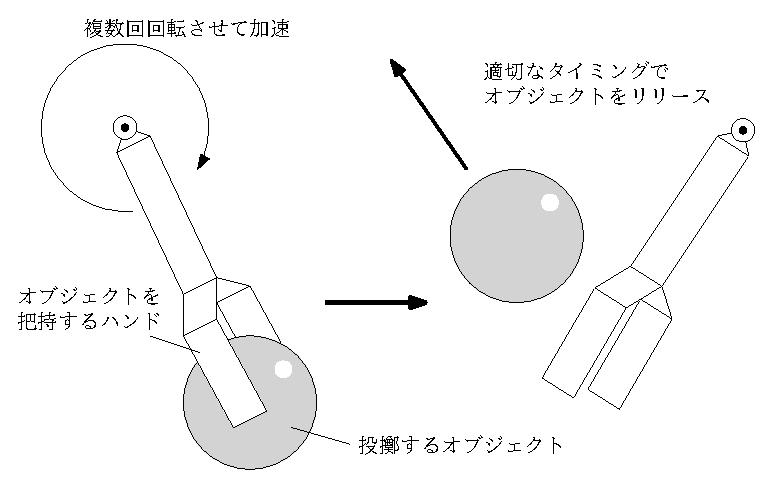
\includegraphics[width=12.5cm]{mecha/fig/rotate.eps}
  \caption{回転アーム型の射出機構}
  \label{fig:rotate}
\end{figure}

尚, このアームを1回転未満で運用する場合は急加速, 急減速を必要とするため, 直動カタパルト型の機構特徴を持つのでそちらを参照してください.
\section{基本的な設計指針}
第\ref{mecha:base}章ではロボットの全体構成について説明しました. では実際にロボットを設計していく際にどのような手順を踏んでいけばよいか, 順を追って解説していきます. 
\subsection{アイデアの収集}
どのようなロボットを作る場合においてもアイデアが非常に重要で, これをなくしてロボットを作り始める事はできません. 要するに作り始める前に機体及びその機構のイメージをしっかりと定めなくてはいけません. 
そしてこれは機械においては非常に重要となります. 機械はどうしても制作に時間がかかる上に改良で見込める性能向上は限られているからです. 制作したロボットが求める性能が出なかった場合はまた1から作り直すことが必要となってしまいます. そのため, 1年で結果を出すことを求められるNHKロボコンにおいては良いアイデアを出来るだけ早く得ることが非常に重要となります.

さて, ではどのようにアイデアを得るかが問題となるでしょう. 行いたい動作を達成する機械をどのように構成するかは設計者によって個性が出る部分であり, 同時に性能の差も付きやすい部分です. 行いたい動作の発想自体は悪くなかったとしても, それを実現するためのアイデアが浮かばなければ意味がありません. 
ここで, あまり経験がない人ほど考え込んでしまう場合が多いです. もちろん, 考えることは悪いことではないですが残念ながら天才でもない限りいきなりアイディアが浮かぶということはありません. 
ここで, 実際に作ってみるなどして自分で手を動かしてみることが大事というのが世の中ではよく言われます. これは非常に正しいですし, 最終的にはそうやって得られるアイデアも非常に多いのですが, その前に少しやったほうが良いことがあります. それがアイデア収集です. というのも前述したとおり機械は制作に時間がかかります. 手を動かしてみて作った後にそれから得られた知見をもとに作り直すには限度があります. あと5年位あればもっと良いものが出来ていたのに……という事になりかねません. この作り直しを減らせる可能性があるのが事前のアイデア収集です.

NHKロボコンではルールが毎年変わるために過去のアイデアが全くそのまま用いられるわけではありません. しかしながら, 小さな機構単位であれば役に立つことは多くあります. そのため, 過去のロボコンに出場したロボットを分析してアイデアを収集することはまず行うべきでしょう. 自分のやりたい動作に近い動きをしている部分はないか, どのようにその動作を達成しているか, それは自分たちには可能かを調べて参考にすると良いです. 

また, 世の中に存在する機構からもアイデアを得ることは出来ます. 身の回りに面白い動きをしているものや, 役に立ちそうな機構があればそれを応用することも出来るでしょう. ただし, スケールの違うものはそのまま適応出来ないこともあるのでその点は留意しておく必要があります. 

\subsection{機構の選定}
ある程度アイデアを集めることができたら, 次に必要なのはその取捨選択です. 望ましいのは考えられうるすべての機構を実際に作ってみてその性能を評価することですが, 資金も時間も限られるNHKロボコンにおいてこれは現実的ではない場合もあります. ではこれに対する対応策を考えてみましょう.

よくあるのは勝負を左右する重要な機構においては複数種類作って実験を行い, その性能を評価するが, それ以外の機構については最もうまくいきそうな機構, 場合によっては設計者の好みの機構を採用するという方式です. 
メリットとしてはその競技に最も適していそうな機構を採用することができる点です. 
一方で人や資金, 時間が豊富でないと出来なかったり, 中途半端に終わってしまうことがあるという点はそのような資源が豊富でないチームにおいてはデメリットです. 機構を評価してどの機構に決定するかに長い時間をかけてしまい, 肝心のロボット制作の時間が大きく減ってしまったという話もよく聞かれます. 
また, どのように評価するかを定めておかないと機構の決定が難航する点にも注意しましょう. 評価軸がブレブレであったり, 特定の個人の主観が強く反映された評価軸は適した機構を選定できないばかりか, その後のチーム運営にも大きな悪影響ともなりうるので注意が必要です. 

勝負を左右するような機構も最初から1つの機構に絞ってしまい, それを突き詰めるという方式もあります. 
これはどの機構に絞るかによって最終的なロボットの性能が決定してしまうというデメリットがありますが, チームの人数や資金, 活動時間に制約があるチームではこちらの方式が適していることもあります. 
というのも, NHKロボコンはどのチームも開発期間が1年で, 機構の最適化が完全に行いきれないためです. そのため, あまりその競技やタスクに適していないような機構であっても, しっかり開発できていれば十分に勝負出来ます. 実際に, 機構は全く違うがほとんど同じ成績を出すロボットも毎年多く見られます. これは優勝するようなレベルのロボットに関しても例外ではありません.
ただし, どのような機構であってもしっかり開発すれば優勝を目指せるというわけではありません. ある程度の性能を発揮できる機構であることが前提条件です. そのために, 採用しようとする前に候補となる各機構の調査及び分析を行うことは非常に重要となります. 過去の使用例や, その機構を使用した人の経験談, 過去にその機構を採用した理由や開発経緯など, 様々な観点から情報を集めて判断に役立てると良いでしょう. 

\subsection{アクチュエータの検討}
実際にどのような機構を採用するか決定する前から, 各機構に使用しうるアクチュエータに関してはよく検討する必要があることもあるため, 前項の機構の選定と順番が前後します. 

実際に作りたい機構にどのアクチュエータを使用するかは制御する側にも大きく影響があるためアクチュエータを決定する際には制御担当者とよく話し合う必要があります. 決して機械側の都合だけで決定せず, 制御側の都合も考慮してお互いが納得するように決定するようにしましょう. 

さて, 機械的な観点ではアクチュエータは回転する形で動力を取り出せるものと, 直動の形で動力を取り出せるものの2種類があります. 回転することで動く機構に関しては回転する形で動力を取り出せるアクチュエータ, 直動することで動く機構は直動の形で動力を取り出せるアクチュエータが望ましいですが, 直動と回転は変換が可能なので, あまり大きな問題にはなりません. 直動と回転で違いがあるとすれば減速, 増速のしやすさです. 一般に直動するタイプの機構は大きな減速や増速は行いにくいです. そのため, 必要なトルクや速度を出せるアクチュエータがないと設計が困難となります. 
一方で回転するタイプのアクチュエータはギアなどを使用すれば簡単に増速や減速が行えます. そのため必要なトルクや速度をそのまま出力できるアクチュエータがなかったとしても, 減速機で調整することで必要なトルクや速度を得ることが出来ます. 

アクチュエータの分類として他に, 電気エネルギーで動くか空圧で動くかという分類も考えられます. 例外はあるものの, 電気で動くアクチュエータは各種モーターなど回転する形で動力を取り出せるものが多いです. 空圧で動くアクチュエータはエアシリンダーなど, 直動の形で動力を取り出せるものが多いです. 
電動のアクチュエータを使用するか空圧のアクチュエータを使用するかは制御側の都合も大きく関わるので機械の都合だけで決定はできませんが, 機械側の観点として, 空圧は多くの体積が必要であることを頭に入れておきましょう. 電動アクチュエータは多くの場合バッテリーを1個か2個搭載しておけば試合時間を乗り切ることが出来ますが, 空圧の場合はそうとも限りません. 使用する量が多い場合は大量の空圧タンクを必要とします. NHKロボコンでは空圧タンクとしてペットボトルが用いられる事が多いですが, 使用する空気の量が多いとこのペットボトルを10本以上搭載することが必要な場合もあります. また, 使用すればするほど出力が低下していくことにも気をつけましょう. 出力が一定であることが必要な機構などでは使用に向きません. 
また, 空圧は危険であることもよく頭に入れておく必要があります. そのため, 空圧タンクにダメージが加わらないような設計や, 空圧タンクを守る構造及びスペースも確保しなくてはいけません. これらのスペースについてもアクチュエータを考えるときに気を配るようにしましょう. 
\subsection{その他調整が必要な部位}
ここまでは個々の機構についての設計方針について述べましたが, ロボット全体のバランスを考えて調整が必要な場合があります. 特に, オブジェクトを取得してから投擲したりセットしたりする過程でオブジェクトが複数の機構を経由する場合はそれぞれの機構との調整が欠かせません. お互いの機構が干渉する可能性やオブジェクトをどの向きで受け渡すかなどはよく考えるべきでしょう. また, 機構単体で見ると良い性能であっても, 両方とも搭載すると展開制限を超えてしまうなどの場合もあります. このような場合, そのまま両方とも採用することは出来ないので全体の構成を決める際には注意しましょう. 
他にも, ロボットのどの位置に機構を取り付けるかによっても全体の性能が変わってきます. とりあえず機構さえ搭載しておけばよいというものではないので, それぞれの機構がロボットのどの位置に搭載する必要があるのか, 他にその位置に搭載する必要のある機構がないかも考えつつ設計すると良いでしょう. 

\section{実際に機械を設計及び制作していく際の留意事項}
ここまでは, 各機構の決定及び設計を主眼に解説してきましたが, 実際にロボット全体の設計及び制作を行っていく際には他にも留意すべき事項があります. 
\subsection{回路の搭載}
多くのロボットでは回路がないと動くことは出来ません. 回路は機械を設計する人にとってはあまり馴染みがないものかも知れませんが, 最低限どの程度の大きさがあって, どのように搭載するか, どの位置に設置する必要があるかは知っておきましょう. そして, 回路を載せるスペースを忘れずに設けるようにしましょう. ここでの回路にはセンサーなども含みます. 制御する人からセンサーを搭載してほしいと言われた場合は, どこに搭載するべきか, どのように搭載するかをよく話し合って決定し, 搭載するようにしましょう.
また, 回路だけでなく, モーターやセンサーからはケーブルが出ていることも忘れてはいけません. ケーブルをどこを通すか, ケーブルが機構の邪魔にならないかなども設計の際に頭の片隅には置いておくようにしましょう. 
\subsection{重量}
重量はロボコンにおいては常に付いて回る課題です. NHKロボコンは重量制限が厳しい傾向があり, 注意していないと制限を超えてしまうことも多々あります. 各機構を設計する段階からどの程度の重量を目指すべきか, 機構ごとに大まかな目安を付けて設計していくようにすると良いでしょう. 
例えば, 重量制限が20kgのロボットを設計しようとしたときには, 足回りの目標重量が10kg, アームが2kg, 投擲機構が3kg, 回路(バッテリー含む)が3kg, ペットボトルなど空圧機器が1kg, 余裕が1kgで合計20kgといった具合です. 
これらの目標を達成できるか, 達成できそうにないならどこの重量を削るかを常に考えながら設計, 制作をするようにすると良いでしょう. 
\subsection{各機構の統合}
多くの場合, 1つのロボットを設計する際に, 機構ごとに担当を分担し, それぞれの担当者が設計した後に統合するという方法をとります. この場合, 各機構の設計が終了したあとにそれぞれの機構を統合しようとすると, うまく統合できなかったり統合に多くの時間がかかってしまったりする場合がしばしばあります. 
このような事態を避けるため, 設計を始める前に各機構の大きさや接続方法を可能な限りしっかりと定めておくようにしましょう. 
また, 設計中にもお互いの連携を欠かさず, 想定外のサイズ変更や要件変更などは常に共有する習慣をつけましょう. 
しっかりと連携をとっておけば, 最終的に統合して1つのロボットにするときにも想定外の事態が発生せず, スムーズに統合することができます. 複数人で1つのロボットを作っているという意識を忘れないようにしましょう. 
\subsection{納期}
実際に制作していく際には, 納期は常についてまわる問題です. 機械は部品が届かないと制作が出来ません. 
材料はどこから購入するのか, その場合の納期はどのくらいかは頭に入れて行動するようにしましょう. 例えば, 納期に1週間かかることがわかっていて使う予定のある部品は, 組み立てが始まる1週間より前に発注するなど, 全体として制作が滞るような事のないように気をつけましょう. 
また, 加工にどのくらいの時間がかかるかも頭に入れておく必要があります. 自分たちの使える加工設備の処理能力などからどのくらい加工に時間がかかるかは理解しておくようにしましょう. これらの時間は, 伸びることはあっても, 縮まることはほとんどないということも気をつけなくてはいけません. さらに, 回路の搭載や制御の時間などは機械の設計や制作には関係ありませんが, 最終的なロボットの完成には欠かせないものとなっています. 制御にどの程度の時間が必要かよく話し合い, 制御の時間を圧迫しないように計画を持って制作に行うようにしましょう. 
納期に遅れそうなときは直ちにそのことをチーム全体に共有し, 計画の見直しを行うようにしましょう. 計画の見直しを行わないとなし崩し的に予定が延びていきます. 機械は納期の短縮が難しいことを頭に入れ, 無理のない計画, こまめな見直しを忘れないようにしましょう. 